%% Chapter 5: System design
\chapter{System Design}
\label{chapter:system-design}

\graphicspath{ {report/C5 System Design/assets/} } 

\section{Design of the SSVEP Stimuli}
\label{subsection:ssvep-stimuli}
A key consideration in the design of the SSVEP stimuli is the stimulus frequencies $f_1, \dots, f_n$ to use. As mentioned in Section \ref{subsection:time-frequency-considerations-c2}, similar studies typically use stimulus frequencies between 7Hz and 12Hz for this task. Furthermore, as detailed in Section \ref{subsection:CCA-c2}, CCA and CCA-based decoding algorithms involve a harmonic reference signal set. An important consideration is the \textit{number of harmonics} to include in these reference sets. In order to allow for a fundamental stimulus frequency range of 7Hz to 12Hz, it is only feasible to include one harmonic ($N_h=1$) in the reference set since the second harmonic of a 12Hz stimulus signal would occur at 36Hz which would likely be attenuated somewhat by the analogue low-pass filter (corner frequency of 37.4Hz) and low-pass filter dynamics of the adjustable output amplifier (corner frequency of 36.35Hz) shown in Figure \ref{fig:analogue-system-c4}. Furthermore, including the second harmonic for each stimulus frequency would have significant memory and computation implications. It is for these reasons that only a single harmonic was used in this system (where applicable).

\subsection{SSVEP stimulus interface}

Naturally, an important part of the SSVEP-based BCI system is the SSVEP stimuli which are to be presented to individuals participating in the exhibition (or in general, anyone interacting with the system thereafter). Taking into account design parameters such as stimulus colour, position and contrast mentioned in the literature cited in Section \ref{subsection:evoking-measuring-ssveps}, a basic user interface (UI) was designed with a series of flashing squares as depicted in Figure \ref{fig:ssvep-squares-c5}. This UI was implemented\footnote{code implementation available \href{https://github.com/JamesTev/EEG-decoding/blob/master/ui/ssvep_squares.html}{here}.} as a lightweight HTML page with basic CSS styling and Javascript to handle animation (flickering of the squares). This decision was made to allow for the simplest and most convenient deployment across any device capable of displaying a web page (mobile or otherwise). The number of blocks being displayed and their labels are subject to adjustment in accordance with other elements of the demonstration beyond the scope of this project.

\begin{figure}[!htb]
    \centering
    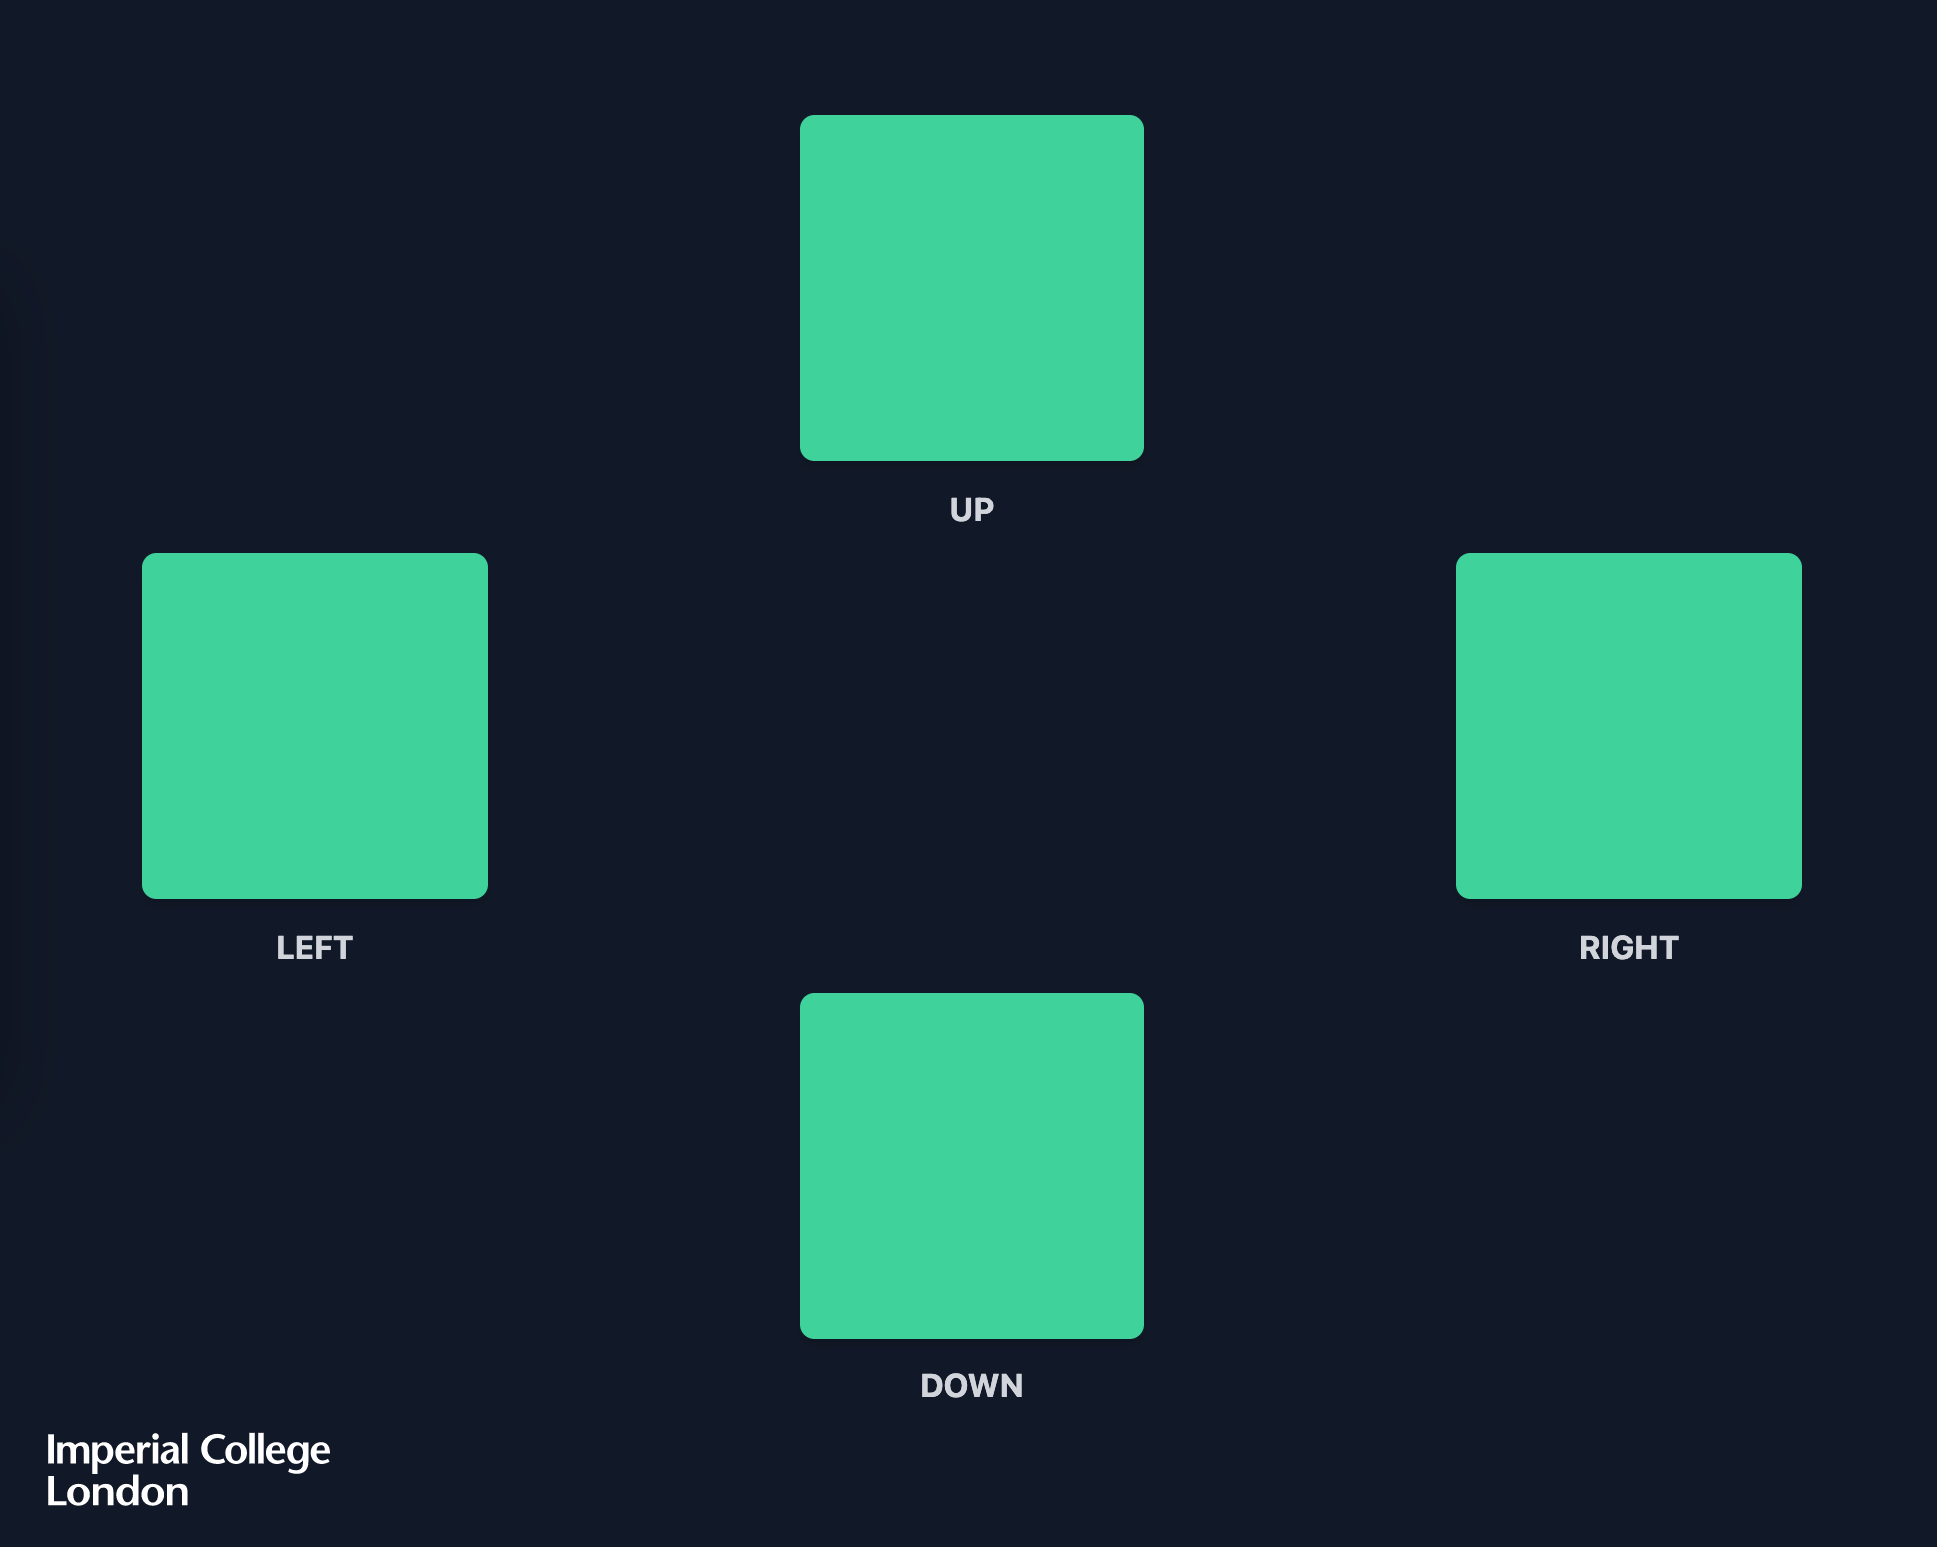
\includegraphics[width=0.7\textwidth]{ssvep-squares}
    \caption{Screen capture of the user interface for displaying SSVEP stimuli. The blocks can be independently set to any flicker frequency of interest.}
    \label{fig:ssvep-squares-c5}
\end{figure}

Note that, external factors related to this project may only require some subset of the stimuli shown in Figure \ref{fig:ssvep-squares-c5}; for example, the square corresponding to `down' may be omitted if only the other three actions are required in the game/simulation. 

\section{Design of the Digital System}
\begin{figure}[!htb]
    \centering
    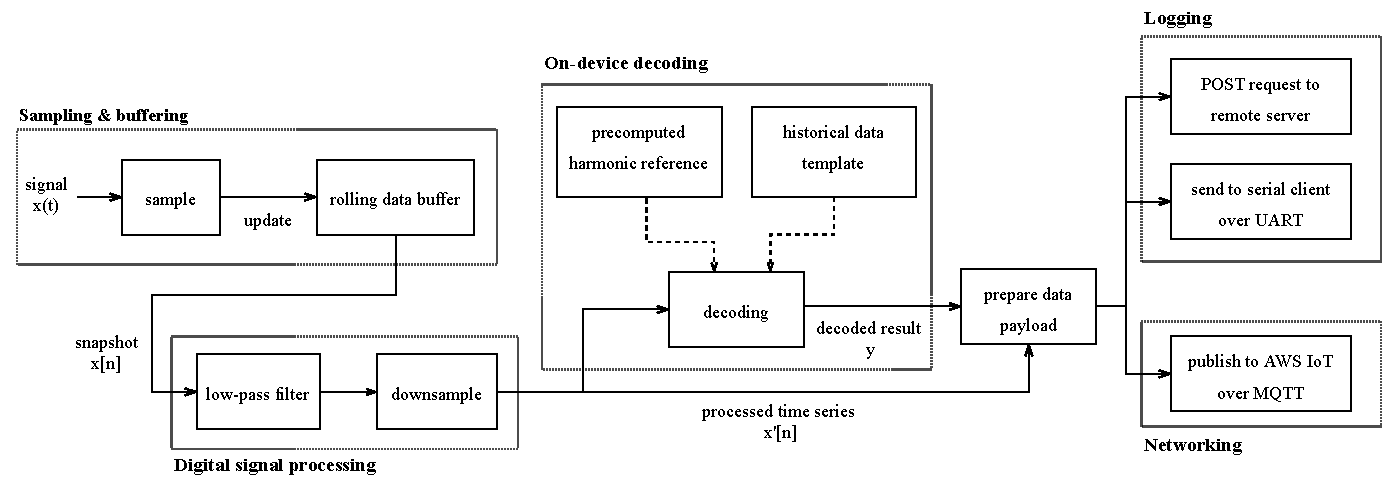
\includegraphics[width=\textwidth]{digital-system-overview}
    \caption{Overview diagram of the core components that comprise the digital system designed in this project.}
    \label{fig:digital-system-overview-c5}
\end{figure}


\subsection{Digital signal processing system}

A crucial part in the design of the BCI system is the digital signal processing (DSP) system. The key functions of this system are to digitise, filter and resample the analogue output of the analogue signal processing system presented in Figure \ref{fig:analogue-system-c4}. An overview of the DSP system is shown in Figure \ref{fig:digital-system-c5}.

\begin{figure}[!htb]
    \centering
    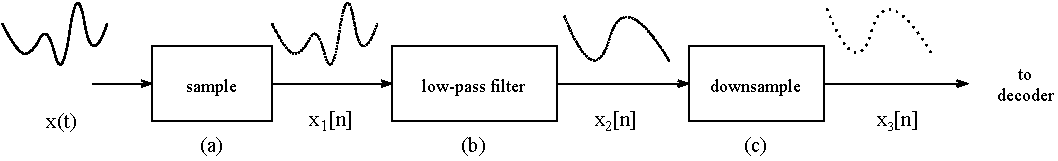
\includegraphics[width=0.9\textwidth]{digital-system}
    \caption[Digital signal processing system]{Overview diagram of the core components of the digital signal processing system.}
    \label{fig:digital-system-c5}
\end{figure}

\subsubsection{Sampling and decimation}
The analogue signal $x(t)$ is digitised to $x_1[n]$ using the 12-bit SAR ADC on-board the ESP32. A sampling frequency of $f_s=256$Hz was selected based for several reasons. First, this is a typical value mentioned in the literature as noted in Section \ref{subsection:time-frequency-considerations-c2}. Second, and more importantly, considering the SSVEP stimulus frequency band of 6 - 12Hz as mentioned in Section \ref{subsection:ssvep-stimuli}, and allowing for one reference signal harmonic in CCA-based decoding algorithms, the maximum theoretical frequency required is $f_{\textrm{max}}=24$Hz. In order to satisfy the Nyquist sampling criterion, sampling at $f_s > 2f_{\textrm{max}} = 48$Hz is required. 64Hz was identified as an appropriate fit as it provides some frequency margin for filter roll-off and it is a factor of 256Hz which facilitates decimation by an integer factor.

\begin{figure}
    \centering
    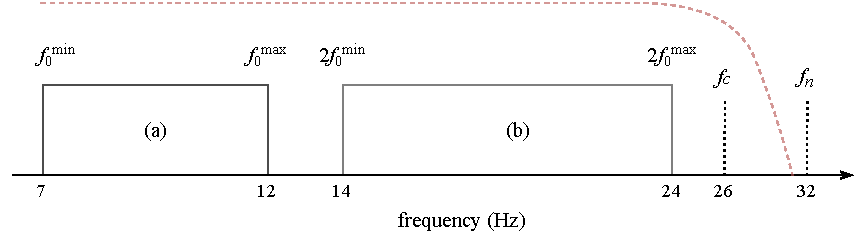
\includegraphics[width=0.85\textwidth]{ssvep-bands}
    \caption[Diagram showing SSVEP stimulus frequency bands and other important frequencies]{Diagram showing SSVEP stimulus frequency bands and other important frequencies. Band (a) represents the fundamental stimulus frequency range and (b) represents the range of first harmonics thereof. The dotted red line is an indicative (idealised) low-pass filter response with corner frequency at $f_c=26$Hz. Including a small safety margin to allow for filter roll-off, $f_n$ represents the Nyquist frequency for this configuration.}
    \label{fig:ssvep-bands}
\end{figure}

Figure \ref{fig:ssvep-bands} shows a high-level view of the sampling and filtering requirements of the system taking into account EEG and SSVEP dynamics, as well as restrictions specific to this project such as memory constraints. 

\subsubsection{Digital filtering}
As indicated in Figure \ref{fig:ssvep-bands}, an ideal low-pass filter for this system would achieve zero pass-band distortion (ripple) between 7 and $24$Hz and steep roll-off after $f_c=26$Hz to achieve complete signal attenuation before the Nyquist frequency $f_n=32$Hz. Obviously, this is not physically realisable and so a trade-off between maximising filter roll-off and minimising pass-band ripple must be sought.  

Infinite impulse response (IIR) filters are typically more suitable for small, resource-constrained DSP systems. Compared to finite impulse response (FIR) filters, they generally offer:
\begin{itemize}
    \item the ability to be implemented recursively
    \item greater computational efficiency
    \item lower memory requirements
    \item improved resolution at lower frequencies
\end{itemize}
Although FIR filters typically offer greater stability and controllability owing to only having zeros in their transfer functions, the aforementioned benefits of IIR filters were deemed to be more important for this application. 

Figure \ref{fig:digital-filt-resp} shows the frequency response of three different commonly used IIR digital filters: type I and II Chebyshev filters, as well an elliptical filter. Each of these filters were designed to meet the following requirements:
\begin{itemize}
\label{list:filter-design-reqs}
    \item maximum filter order of $n=10$
    \item maximum pass-band ripple (below unity gain) of $r_p=0.2$dB 
    \item minimum stop-band attenuation of $r_s=80$dB
\end{itemize}

\begin{figure}[h]
    \centering
    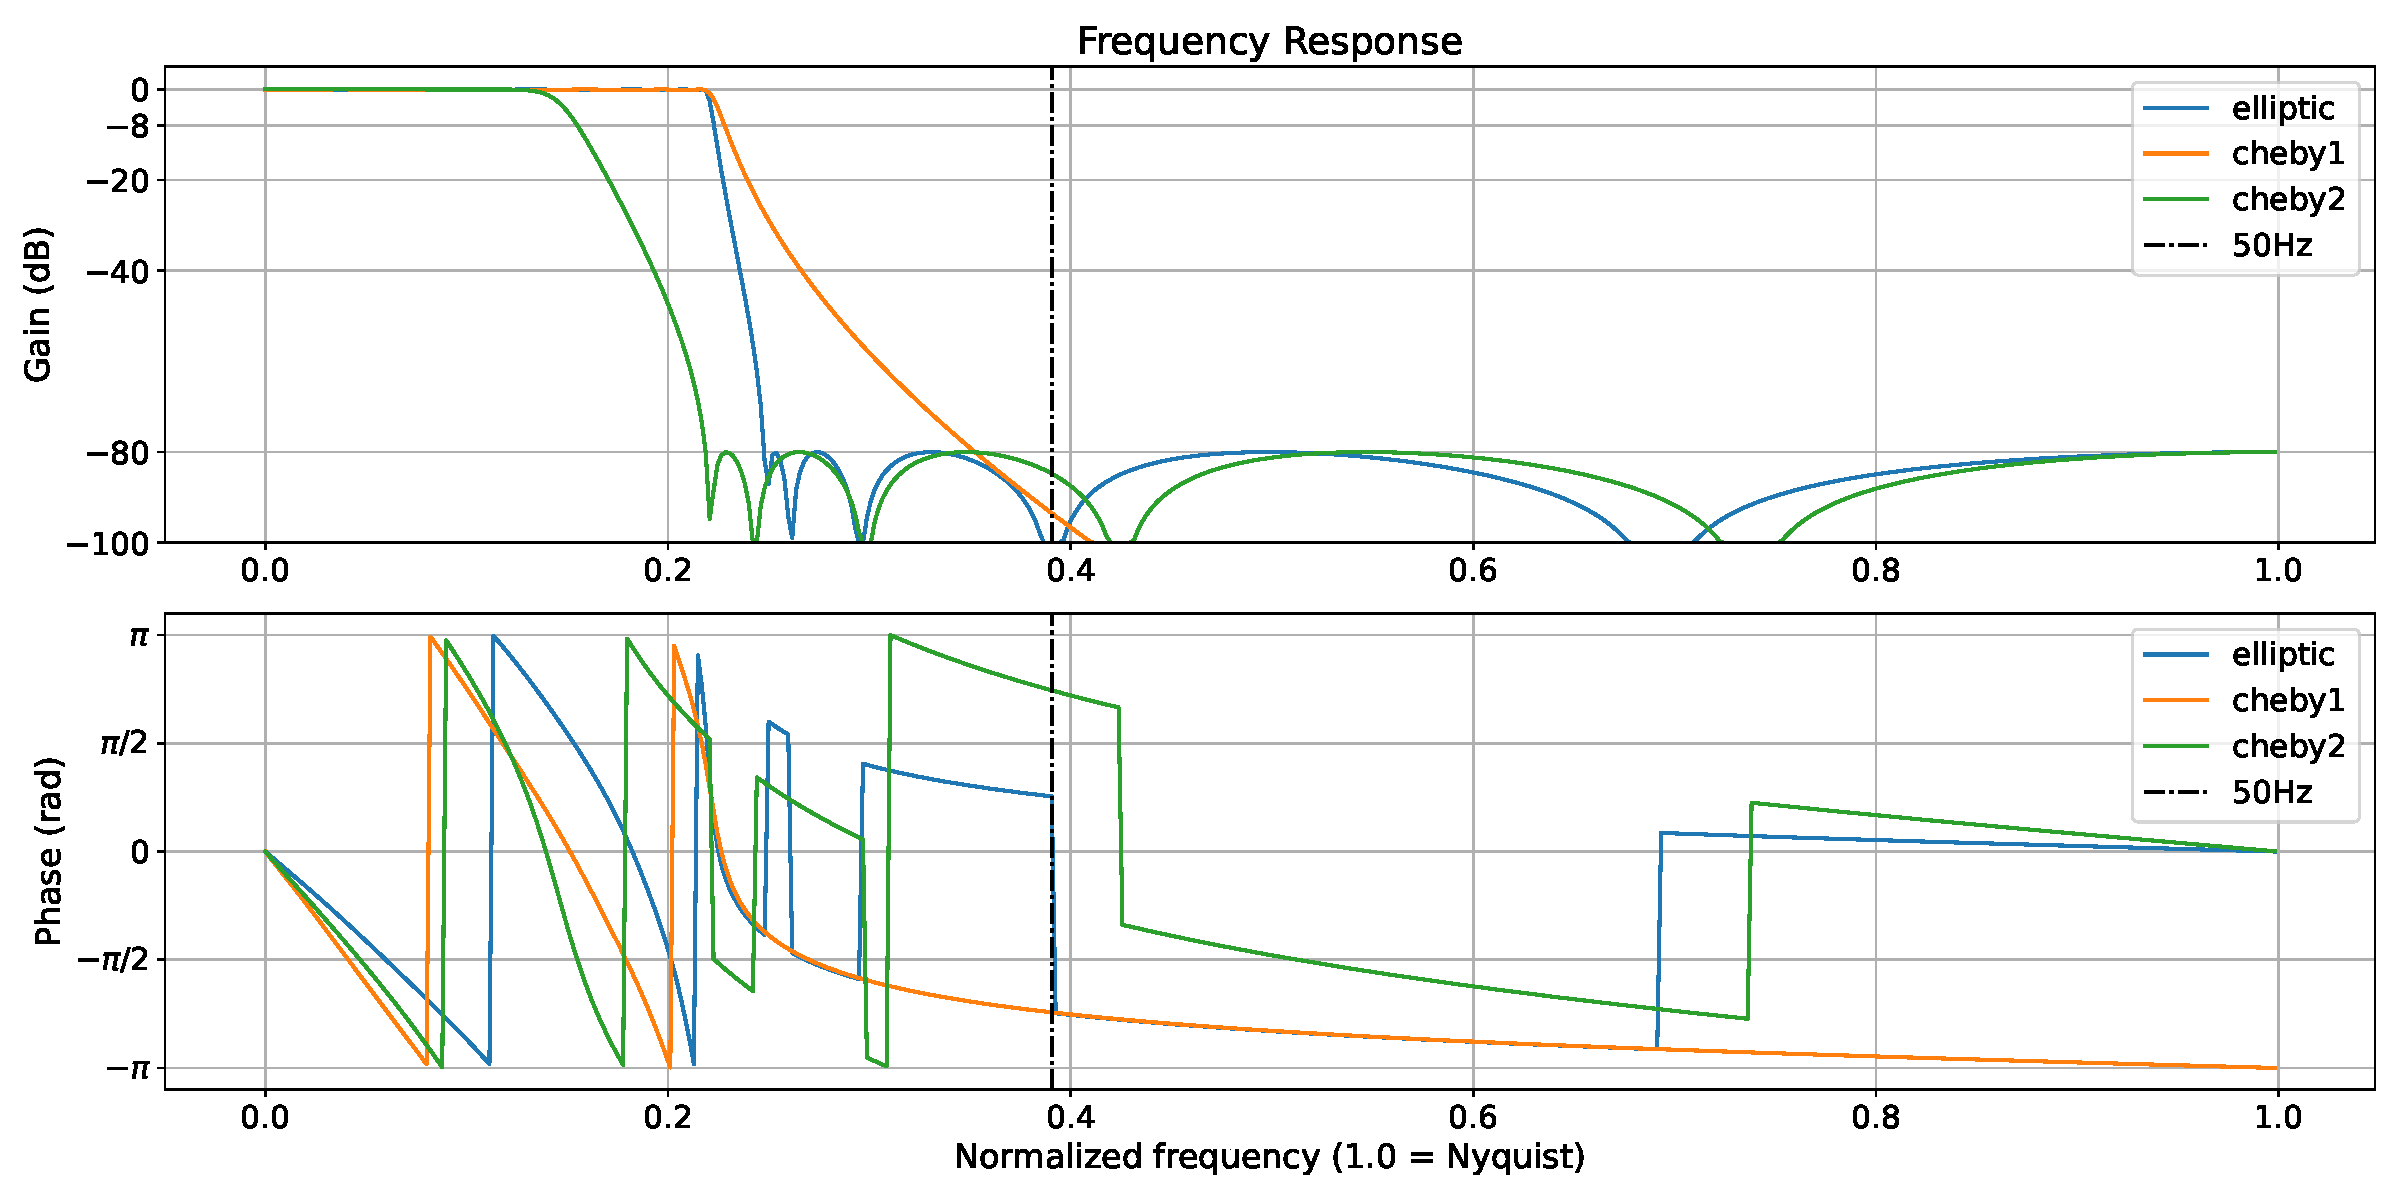
\includegraphics[width=\textwidth]{digital-filt-resp}
    \caption[Frequency response of the digital low-pass filter implemented in firmware on the ESP32]{Frequency response of the digital low-pass filter implemented in firmware on the ESP32. The pre-filtered Nyquist frequency in this implementation is 128Hz: half the 256Hz sampling frequency.}
    \label{fig:digital-filt-resp}
\end{figure}
Observing the magnitude plot in the to half of Figure \ref{fig:digital-filt-rep}, it is evident that the response of the elliptic filter offers the optimal balance of steep roll-off between pass and stop bands and acceptable ripple in the stop and pass bands. This is intuitive: as $r_p$ approaches zero, the elliptical filter becomes a Chebyshev type II filter. As $r_s$ approaches zero, it becomes a Chebyshev type I filter. The phase response of the elliptical filter is also largely linear in the pass-band. For these reasons, a $10^{\textrm{th}}$ order elliptical low-pass filter satisfying the aforementioned design requirements was selected.

\section{Embedded Firmware}
As alluded to in Section \ref{subsection:electronic-hardware-proto}, all firmware for this system was to be developed for the ESP32 SoC developed by Espressif Systems. Espressif offers a comprehensive \href{https://github.com/espressif/esp-idf}{open source} framework called the Espressif IoT Development Framework (ESP-IDF) that can be used to develop ESP32-based applications on Windows, Linux and macOS using C and C++ programming languages. Furthermore, ESP-IDF tooling has been extended to be used with the popular open source platform Arduino. While the ESP-IDF has arguably become the de facto standard for developing complex embedded applications for the ESP32, a different approach was taken in this project for reasons explored below. 

\subsection{MicroPython}
MicroPython is a lean and highly efficient implementation of the Python 3 language that provides a carefully-selected subset of the Python standard library that is optimised for microcontrollers and other resource-constrained targets \cite{micropython}. In fact, MicroPython is a full Python compiler and runtime implemented in C (C99) that runs natively (on bare metal) on several architectures. It is an open source project started by Damien George in 2013 that has since gained great traction from the open source community with constant feature updates and fixes. Some of its notable features include \cite{micropython}: 
\begin{enumerate}
    \item compact enough to fit and run within 256k of ROM (code space) and 16k of RAM.
    \item many different compile-time configuration options
    \item support for many architectures (both for microcontrollers and fully-fledged microprocessors): x86, x86-64, ARM, ARM Thumb, Xtensa
    \item inline assembler for Thumb and Xtensa instruction sets
    \item a cross-compiler that allows ordinary Python scripts to be cross-compiled into bytecode that can be loaded from non-volatile flash instead of RAM.
    \item explicit memory errors (\texttt{MemoryError}) for heap exhaustion
    \item explicit run time errors (\texttt{RuntimeError}) when reaching the stack limit
\end{enumerate}

The technical features of MicroPython listed above have some very useful practical implications for application development on the ESP32 that are not available when developing using the ESP-IDF in C/C++. Practical advantages of MicroPython include:
\begin{itemize}
    \item The convenience of using the Python programming language which offers far more high-level functions and constructs over C or C++.
    \item A real-time interactive Python prompt (REPL) that allows commands to be tested and executed immediately over a serial connection. For some MicroPython ports, including that of the ESP32, a WebREPL is also provided that allows for interactivity over a wireless network connection.
    \item Support for both microcontroller and desktop architectures such as X86 allows MicroPython code to be tested with exact equivalence on a personal computer without having to interact with a microcontroller. This can be very useful for prototyping and algorithm development.
    \item A very familiar and intuitive micro-directory and module structure that emulates regular Python modules (explored more below).
    \item A community of open source developers that can very easily contribute new modules and peripheral functionality 
\end{itemize}

\subsection{Module structure}
As alluded to above, a very convenient feature of MicroPython is its intuitive module/file structure. It allows python modules in the form of \texttt{.py} files to be organised in folders that serve as packages as with regular Python. This file structure is stored directly in flash storage on the device and can be read or written to at any time during development. Consider the module structure of the MicroPython application developed in this project below:

\dirtree{%
.1 /.
.2 boot.py.
.2 main.py.
.2 .env.
.2 lib.
.3 core.py.
.3 decoding.py.
.3 peripherals.py.
.3 \dots.
.2 certificates.
.3 dab0ac2b5c-private.pem.key.
.3 dab0ac2b5c-public.pem.key.
.3 dab0ac2b5c-certificate.pem.crt.
.2 logs.
.3 log-17082021-1.json.
.3 log-10072021.txt.
}
The root directory contains two important files - \texttt{boot.py} and \texttt{main.py} - that are run in sequence at boot time. The \texttt{boot.py} script is typically used for internal system processes and \texttt{main.py} is used for any user functionality that should automatically be run at boot. Also in the root directory is the \texttt{.env} file which can be used to store sensitive environment variables such as Wi-Fi passwords or API key strings. The \texttt{lib} directory (package) contains the modules that implement the actual functionality of the digital system, including peripheral management, decoding and computation and networking (note that not all modules are shown above). Amazon AWS key files and certificates for secure MQTT communication are stored in the \texttt{certificates} folder. Finally, a \texttt{logs} directory shows how log files can also be very conveniently stored in arbitrary formats such as \texttt{.json} or \texttt{.txt} in non-volatile flash memory. Listing \ref{listing:dir-structure} below demonstrates how user-specific modules and files can be imported and used within a new script once flashed to the microcontroller's non-volatile memory. 

\begin{listing}[h]
\begin{minted}{python}
# import user-specific functions from non-volatile memory
from lib.decoding import cca
from lib.computation import solve_gen_eig_prob as solve_eig

# MicroPython emulation of the standard Python `os` module
import os

# list root directory
print(os.listdir('/'))

# open and read a file from flash
with open('/logs/log-10072021.txt') as f:
    print(f.read())
\end{minted}
\caption[Basic MicroPython code to import user-specific modules and read from a text file in non-volatile storage.]{Basic MicroPython code to import user-specific modules and read from a text file in non-volatile storage. Note that the syntax is identical to ordinary Python.}
\label{listing:dir-structure}
\end{listing}

\subsection{Numerical computation}
An additional important motivation for using MicroPython over the more traditional C/C++ approach is the ability to use an extremely convenient open source MicroPython module called \texttt{ulab}\footnote{Source code and documentation available \href{https://github.com/v923z/micropython-ulab}{here}.} The \texttt{ulab} project was created to offer a subset of the very popular \texttt{numpy} numerical computing library for Python which offers highly performant array computing and linear algebra functionality. It also implements a small subset of functionality offered by \textt{scipy}; the equally popular scientific computing library for Python. Some of the most notable features offered by this module include \cite{ulab}:
\begin{enumerate}
    \item compact, iterable and sliceable arrays structures for numerical data up to 4 dimensions
    \item extremely frugal with RAM usage
    \item efficient, vectorised computations on multi-dimensional arrays
    \item basic linear algebra functionality such as matrix inversion, multiplication, determinants, Cholesky and QR decomposition
    \item fast Fourier transforms (FFTs)
    \item implementation of digital filters using second order sections (SOS)
    \item basic numerical approximation and function minimisation
\end{enumerate}
Being able to perform matrix and array operations, filtering and numerical approximation on a microcontroller in an elegant, Pythonic way is clearly an invaluable asset for this project. Indeed, for any project of this sort, it is somewhat amazing. Listing \ref{listing:ulab-intro} briefly demonstrates just how effortlessly complex numerical computations can be performed using \texttt{ulab}.

\begin{listing}[h]
\begin{minted}{python}
# import ulab module
from ulab import numpy as np

# create an arbitrary positive definite, symmetric 3x3 matrix
# A can be sliced like A[i0:i1, j0:j1]
A = np.array([[25, 15, -5], [15, 18,  0], [-5,  0, 11]])

# compute lower triangular square root or A using Cholesky decomp
A_sqrt = np.linalg.cholesky(A)

# compute determinant of A
det_A = np.linalg.det(A)

# compute inverse of A
A_inv = np.linalg.inv(A)

# compute Moore-Penrose pseudoinverse of A = (A^T.A)^-1.A^T
A_pinv = np.dot(np.linalg.inv(np.dot(np.transpose(A), A)), np.transpose(A))

# many other utility functions such as argmax(), argsort(), convolve()

\end{minted}
\caption{Illustration of the convenience offered by the \texttt{ulab} module for linear algebra and general numerical computing}
\label{listing:ulab-intro}
\end{listing}

\subsection{Networking}
Discuss AWS IoT interface and real-time streaming capabilities using MQTT

\begin{figure}[!htb]
    \centering
    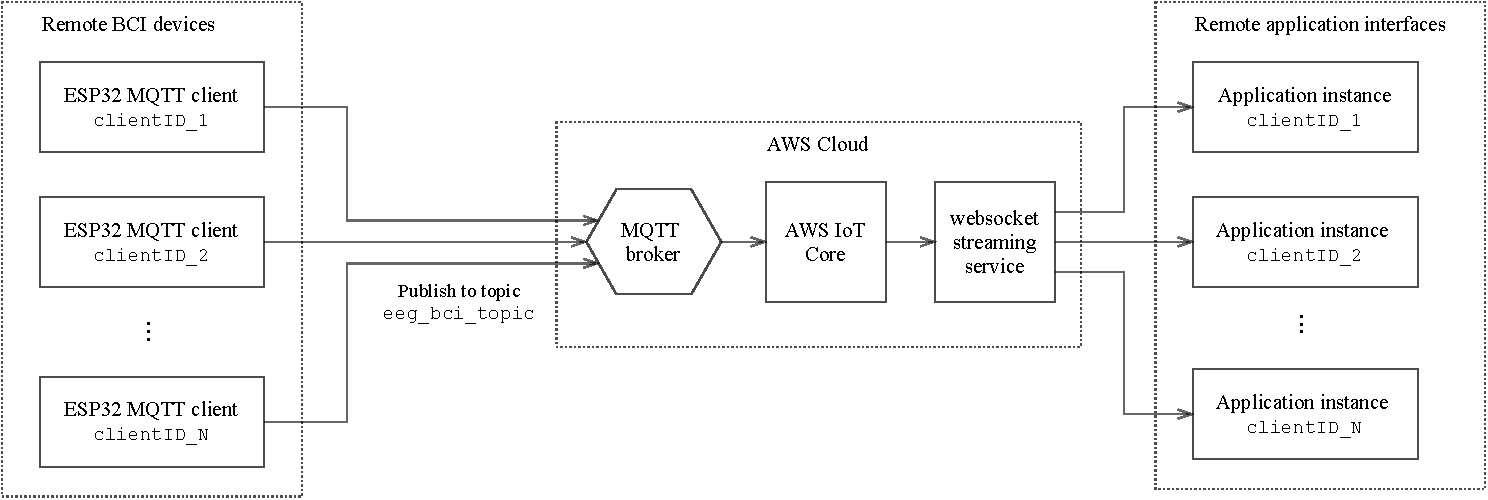
\includegraphics[width=\textwidth]{network-diagram}
    \caption{Networking diagram}
    \label{fig:networking-diagram-c5}
\end{figure}


\section{Algorithm Implementation}

\begin{algorithm}[H]
\DontPrintSemicolon
  
  \KwInput{Your Input}
  \KwOutput{Your output}
  \KwData{Testing set $x$}
  $\sum_{i=1}^{\infty} := 0$ \tcp*{this is a comment}
  \tcc{Now this is an if...else conditional loop}
  \If{Condition 1}
    {
        Do something    \tcp*{this is another comment}
        \If{sub-Condition}
        {Do a lot}
    }
    \ElseIf{Condition 2}
    {
    	Do Otherwise \;
        \tcc{Now this is a for loop}
        \For{sequence}    
        { 
        	loop instructions
        }
    }
    \Else
    {
    	Do the rest
    }
    
    \tcc{Now this is a While loop}
   \While{Condition}
   {
   		Do something\;
   }

\caption{Example code}
\end{algorithm}


Discuss numerical challenges, precision issues, memory constraints
Discuss some of the auxiliary computational approaches used such as eigenvalue solvers etc

